% Dokumentklassen sættes til memoir.
% Manual: http://ctan.org/tex-archive/macros/latex/contrib/memoir/memman.pdf
\documentclass[a4paper,10pt,fleqn]{article}
\usepackage[a4paper]{geometry}
% Danske udtryk (fx figur og tabel) samt dansk orddeling og fonte med

% danske tegn. Hvis LaTeX brokker sig over æ, ø og å skal du udskifte
% "utf8" med "latin1" eller "applemac".
\usepackage[utf8]{inputenc}
%\usepackage[danish]{babel}
\usepackage[T1]{fontenc}
\usepackage{fixltx2e}
\usepackage{color}
\usepackage{hyperref}

% Matematisk udtryk, fede symboler, theoremer og fancy ting (fx kædebrøker)
\usepackage{amsmath,amssymb}
\usepackage{stmaryrd}
\usepackage{bm}
\usepackage{amsthm}
\usepackage{tikz}
\usetikzlibrary{arrows}
\usetikzlibrary{positioning}
\usetikzlibrary{snakes}
\usetikzlibrary{decorations.pathreplacing}
\usepackage{mathtools}
\usepackage[makeroom]{cancel}
% Manual: http://mirror.ctan.org/macros/latex/contrib/listings/listings.pdf
\usepackage{listings}
\usepackage{verbatim}
\usepackage{enumitem}
\usepackage{bussproofs}
\usepackage{mathpartir}

% Indsættelse af grafik.
\usepackage{graphicx}
\usepackage{xcolor}
\usepackage{multirow}

%\setlength{\mathindent{0cm}}

\newcommand{\sem}[1]{\ensuremath{\llbracket #1 \rrbracket}}
\newcommand{\tuple}[1]{\ensuremath{\langle #1 \rangle}}
\newcommand{\curly}[1]{\ensuremath{\mathcal{#1}}}

\DeclareMathOperator{\FTV}{FTV}
\DeclareMathOperator{\Rel}{Rel}
\DeclareMathOperator{\dom}{dom}
\DeclareMathOperator{\safe}{safe}
\DeclareMathOperator{\irred}{irred}
\DeclareMathOperator{\SNPred}{SN}
\DeclareMathOperator{\val}{Val}
\DeclareMathOperator{\fst}{fst}
\DeclareMathOperator{\snd}{snd}
\DeclareMathOperator{\inl}{inl}
\DeclareMathOperator{\inr}{inr}
\DeclareMathOperator{\scase}{case}
\DeclareMathOperator{\caseof}{of}
\DeclareMathOperator{\fold}{fold}
\DeclareMathOperator{\unfold}{unfold}
\DeclareMathOperator{\epack}{pack}
\DeclareMathOperator{\eunpack}{unpack}
\DeclareMathOperator{\eas}{as}
\DeclareMathOperator{\ein}{in}
\DeclareMathOperator{\enot}{not}

\newcommand{\pack}[3]{\ensuremath{\epack \; \tuple{#1,#2} \; \eas \; #3}}
\newcommand{\unpack}[4]{\ensuremath{\eunpack \; \tuple{#1,#2} = #3 \; \ein \; #4 }}

\newcommand{\evalto}{\ensuremath{\mapsto}}
\newcommand{\evaltos}[1][*]{\ensuremath{\evalto^{#1}}}
\newcommand{\warning}[1]{{\color{red} !` #1 !} \\}
\newcommand{\mtenv}{{\raisebox{1.5pt}{$\scriptstyle\bullet$}}}
\newcommand{\case}[1]{\\{\bf Case} #1,}
\newcommand{\eqdef}{\ensuremath{ \; \stackrel{\mathclap{\normalfont\mbox{def}}}{=} \;}}
\newcommand{\subst}[3]{\ensuremath{\ensuremath{#1[^{\textstyle #2}/_{\textstyle #3}]}}}
\newcommand{\labs}[2]{\ensuremath{\lambda #1 . \; #2}}
\newcommand{\tlabs}[3]{\ensuremath{\lambda #1 : #2 . \; #3}}
\newcommand{\tLabs}[2][\alpha]{\ensuremath{\Lambda #1 . \; #2}}
\newcommand{\vbar}{\ensuremath{\; | \;}}
\newcommand{\tarrow}[2]{\ensuremath{ #1 \rightarrow #2}}
\newcommand{\eif}[3]{\ensuremath{ \text{if}\; #1 \; \text{then} \; #2 \; \text{else} \; #3}}
\newcommand{\true}{\ensuremath{\text{true}}}
\newcommand{\false}{\ensuremath{\text{false}}}
\newcommand{\SN}[2]{\ensuremath{\SNPred_{#1}(#2)}}
\newcommand{\pand}{\ensuremath{\; \wedge \;}}



\newcommand{\pred}[2]{\ensuremath{\curly{#1}\sem{#2}}}
\newcommand{\pres}[3]{\ensuremath{\curly{#1}_{#2}\sem{#3}}}
\newcommand{\prep}[3]{\ensuremath{\curly{#1}\sem{#3}_{#2}}}

\newcommand{\epred}[1]{\pred{E}{#1}}
\newcommand{\epres}[2][k]{\pres{E}{#1}{#2}}
\newcommand{\eprep}[2][\rho]{\prep{E}{#1}{#2}}

\newcommand{\vpred}[1]{\pred{V}{#1}}
\newcommand{\vpres}[2][k]{\pres{V}{#1}{#2}}
\newcommand{\vprep}[2][\rho]{\prep{V}{#1}{#2}}

\newcommand{\gpred}[1]{\pred{G}{#1}}
\newcommand{\gpres}[2][k]{\pres{G}{#1}{#2}}
\newcommand{\gprep}[2][\rho]{\prep{G}{#1}{#2}}

\newcommand{\dpred}[1]{\pred{D}{#1}}

\newcommand{\sub}[3]{\subst{#1}{#2}{#3}}
\newcommand{\extsub}[3]{\ensuremath{#1 \lbrack #2 \mapsto #3 \rbrack}}

\newcommand{\equivalence}[3]{\ensuremath{#1 \approx^{#2} #3}}
\newcommand{\ctxeq}[2]{\equivalence{#1}{ctx}{#2}}
\newcommand{\lreq}[2]{\equivalence{#1}{LR}{#2}}




\newcommand*{\circled}[1]{\tikz[baseline=(char.base)]{
            \node[shape=circle,draw,inner sep=1pt] (char) {#1};}}


\newcommand{\TTrue}{\ensuremath{
    \inferrule*[right=T-True]{ }
               {\Gamma \vdash \true : bool}}}

\newcommand{\TFalse}{\ensuremath{
    \inferrule*[right=T-False]{ }
               {\Gamma \vdash \false : bool}}}
\newcommand{\TVar}{\ensuremath{
    \inferrule*[right=T-Var]{\Gamma(x) = \tau}
                            {\Gamma \vdash x : \tau}}}
\newcommand{\TIf}{\ensuremath{
    \inferrule*[right=T-If]{\Gamma \vdash e : bool \and \Gamma \vdash e_1 : \tau \and \Gamma \vdash e_2 : \tau}
               {\Gamma \vdash \eif{e}{e_1}{e_2} : \tau}}}
\newcommand{\TApp}{\ensuremath{
    \inferrule*[right=T-App]{\Gamma \vdash e_1 : \tarrow{\tau_2}{\tau} \and
                            \Gamma \vdash e_2 : \tau_2}
                           {\Gamma \vdash e_1 \; e_2 : \tau}}}

\newcommand{\TAbs}{\ensuremath{\inferrule*[right=T-Abs]{\Gamma, x: \tau_1 \vdash e : \tau_2}
                           {\Gamma \vdash \tlabs{x}{\tau_1}{e} : \tarrow{\tau_1}{\tau_2}}}}
\newcommand{\TFold}{\ensuremath{
    \inferrule*[right=T-Fold]{\Gamma \vdash e : \tau[\mu\alpha. \; \tau/\alpha]}
                             {\Gamma \vdash \fold \; e : \mu\alpha. \; \tau}}}
\newcommand{\TUnfold}{\ensuremath{
    \inferrule*[right=T-Unfold]{\Gamma \vdash e : \mu\alpha. \; \tau}
                               {\Gamma \vdash \unfold \; e : \tau[\mu\alpha. \; \tau/\alpha]}}}


\newcommand{\FTTrue}{\ensuremath{
    \inferrule*[right=T-True]{ }
               {\Delta ; \Gamma \vdash \true : bool}}}

\newcommand{\FTFalse}{\ensuremath{
    \inferrule*[right=T-False]{ }
               {\Delta ; \Gamma \vdash \false : bool}}}

\newcommand{\FTVar}{\ensuremath{
    \inferrule*[right=T-Var]{\Gamma(x) = \tau}
                            {\Delta ; \Gamma \vdash x : \tau}}}
\newcommand{\FTApp}{\ensuremath{
    \inferrule*[right=T-App]{\Delta ; \Gamma \vdash e_1 : \tarrow{\tau_2}{\tau} \and
                            \Delta ; \Gamma \vdash e_2 : \tau_2}
                           {\Delta ; \Gamma \vdash e_1 \; e_2 : \tau}}}

\newcommand{\FTAbs}{\ensuremath{
    \inferrule*[right=T-Abs]{\Delta ; \Gamma, x: \tau_1 \vdash e : \tau_2}
                           {\Delta ; \Gamma \vdash \tlabs{x}{\tau_1}{e} : \tarrow{\tau_1}{\tau_2}}}}
\newcommand{\FTIf}{\ensuremath{
    \inferrule*[right=T-If]{\Delta ; \Gamma \vdash e : bool \and
                            \Delta ; \Gamma \vdash e_1 : \tau \\
                            \Delta ; \Gamma \vdash e_2 : \tau}
               {\Delta ; \Gamma \vdash \eif{e}{e_1}{e_2} : \tau}}}
\newcommand{\FTtApp}{\ensuremath{
    \inferrule*[right=T-TAbs]{\Delta,\alpha;\Gamma \vdash e : \tau}
                             {\Delta; \Gamma \vdash \tLabs{e} : \forall \alpha.\tau}}}
\newcommand{\FTtAbs}{\ensuremath{
    \inferrule*[right=T-TApp]{\Delta; \Gamma \vdash e : \forall \alpha . \tau \and
                              \Delta \vdash \tau'}
                             {\Delta ; \Gamma \vdash e [\tau'] : \subst{\tau}{\tau'}{\alpha}}}}


\newtheorem*{theorem}{Theorem}
\newtheorem*{lemma}{Lemma}
%Lecture 1:
\newtheorem*{strnorm}{Theorem}
\newtheorem*{astrnorm}{Theorem}
\newtheorem*{substlem}{Lemma}
\newtheorem*{forback}{Lemma}
%Lecture 2:
\newtheorem*{stlctypesafety}{Theorem}
\newtheorem*{progress}{Lemma}
\newtheorem*{preservation}{Lemma}
\newtheorem*{btypesafety}{Theorem}
%Lecture 3:
\newtheorem*{stlcmutypesafety}{Theorem}
\newtheorem*{stlcmufundprop}{Theorem}
\newtheorem*{monotonicity}{Lemma}
%Lecture 4:
\newtheorem*{fundamentalprop}{Theorem}

\author{Lau Skorstengaard\\lask@cs.au.dk}
\title{OPLSS15, Notes for Amal Ahmed's lectures.}
\begin{document}
\maketitle The videos of the lectures at OPLSS 2015 can be found at \url{https://www.cs.uoregon.edu/research/summerschool/summer15/curriculum.html}.
\section*{Lecture 1, Logical Relations}
\subsection*{Simply Typed Lambda Calculus (STLC)}
Types:
\[
    \tau ::=  bool \vbar \tarrow{\tau}{\tau}
\]
Terms:
\[
    e    ::= x \vbar \true 
                 \vbar \false 
                 \vbar \eif{e}{e}{e} 
                 \vbar \tlabs{x}{\tau }{e}
                 \vbar e \; e
\]
Values:
\[
    v    ::= \true \vbar \false \vbar \tlabs{x}{\tau}{e}
\]
Evaluation contexts:
\[
    E    ::= [] \vbar \eif{E}{e}{e} \vbar E \; e \vbar v \; E
\]
Evaluations:
\begin{align*}
  & \eif{\true}{e_1}{e_2} \evalto e_1 \\
  & \eif{\false}{e_1}{e_2} \evalto e_2 \\
  & (\tlabs{x}{\tau}{e}) \; v \evalto \subst{e}{v}{x} \\
  & \inferrule*[]{e \evalto e'}
               {E[e] \evalto E[e']}
\end{align*}
Typing Contexts:
\[
  \Gamma ::= \mtenv \vbar \Gamma , x : \tau
\]
\clearpage
Typing rules:
\[
  \TFalse
\hspace{2cm}
  \TTrue
\]
\[
  \TVar
\hspace{2cm}
  \TIf
\]  
\[
  \TAbs
\]
\[
  \TApp
\]
\subsection*{Logical Relations}
Proof method used to establish properties. Examples:
\begin{itemize}
\item Termination
\item Type safety
\item Equivalence of programs
  \begin{itemize}
  \item Correctness of programs
  \item Representation independence
  \item Parametricity and free theorems, e.g.,
    \[
    f: \forall \alpha. \; \tarrow{\alpha}{\alpha}
    \]
    The program cannot inspect $\alpha$ as it has no idea which type it will be, therefore this function must be $id$.
    \[
    \forall. \; \tarrow{int}{\alpha}
    \]
    A function with this type does not exist (the function would need to return something of type $\alpha$, but it only has something of type $int$ to work with, so it cannot possibly return a value of the proper type).
  \item Security-Typed Languages (for Information Flow Control (IFC))\\
        Example: All types in the code snippet below are labeled with their security level. A type can be labeled with either $L$ for \emph{low} or $H$ for \emph{high}. We do not want any flow from variables with a \emph{high} labeled type to a variable with a \emph{low} labeled type. The following is an example of an invalid \emph{explicit flow} of information:
        \begin{lstlisting}[escapeinside={@}{@}]
  x : int@$^L$@
  y : int@$^H$@
  x = y    //This assignment is illegal.
        \end{lstlisting}
Further, information may leak through a \emph{side channel}. That is the value denotated by a variable with a \emph{low} labeled type depends on the value of a variable with a \emph{high} labeled type. If this is the case we may not have learned the secret value, but we may have learned some information about it. An example of a side channel:
        \begin{lstlisting}[escapeinside={@}{@}]
  x : int@$^L$@
  y : int@$^H$@
  if y > 0 then x = 0 else x = 1
        \end{lstlisting}
How do we then argue a program is secure? Non-interference:
\begin{align*}
  & \vdash P : \tarrow{int^L \times int^H}{int^L} \\
  & P(v_L,v_{1H}) \approx_L P(v_L,v_{2H})
\end{align*}
If we run $P$ with the same \emph{low} value and with two different \emph{high} values, then the \emph{low} result of the two runs of the program should be equal. That is the \emph{low} result does not depend on \emph{high} values.
  \end{itemize}
\end{itemize}
\subsection*{Categories of Logical Relations}
\begin{tabular}{l | l}
  Logical Predicates     & Logical Relations    \\
\hline
  (Unary)                & (Binary)             \\
  $P_\tau(e)$             & $R_\tau(e_1,e_2)$     \\
  - One property         & - Program Equivalence\\ %\footnote{Was not in my notes.}
  - Strong normalization & \\
  - Type safety          & \\
\end{tabular}
\subsection*{Strong Normalization of STLC}
\subsubsection*{A first try on normalization of STLC}
We start with a couple of abbreviations:
\begin{align*}
  e \Downarrow v & \eqdef e \evaltos v \\
  e \Downarrow   & \eqdef \exists v. \; e \Downarrow v
\end{align*}
What we want to prove is:
\begin{strnorm}[Strong Normalization]
  If $\mtenv \vdash e : \tau$ then $e \Downarrow$
\end{strnorm}
\begin{proof} 
\warning{This proof gets stuck and is not complete. It is included to motivate the use of a logical predicate.}
Induction on the structure of the typing derivation.
\case{$\mtenv \vdash \true : bool$} this term has already terminated.
\case{$\mtenv \vdash \false : bool$} same as for \true.
\case{$\mtenv \vdash \eif{e}{e_1}{e_2} : \tau$} simple, but requires the use of canonical forms of bool.
\case{$\mtenv \vdash \tlabs{x}{\tau_1}{e}$ : \tarrow{\tau_1}{\tau_2}} it is a value, it has terminated.
\case{$ \TApp $} \\
By the induction hypothesis we get $e_1 \Downarrow v_1$ and $e_2 \Downarrow v_2$. By the type of $e_1$ we conclude $e_1 \Downarrow \tlabs{x}{\tau_2}{e'}$. What we need to show is $e_1 \; e_2 \Downarrow$.
\begin{align*}
  e_1 \; e_2 & \evaltos (\tlabs{x}{\tau_2}{e'}) \; e_2 \\
            & \evaltos (\tlabs{x}{\tau_2}{e'}) \; v_2 \\
            & \evalto e'[v_2/x]
\end{align*}
Here we run into an issue as we do not know anything about $e'$. Our induction hypothesis is not strong enough.\footnote{:(}
\end{proof}
\subsubsection*{A logical predicate for strongly normalizing expressions}
We want to define a logical predicate, \SN{\tau}{e}. We want $\SNPred_\tau$ to accept the expressions of type $\tau$ that are strongly normalizing, but let us first consider what properties we in general want a logical predicate to have.

In general for a logical predicate, $P_\tau(e)$, we want an expression, $e$, in accepted by this predicate to satisfy the following properties\footnote{Note: when we later want to prove type safety we do not want well-typedness to be a property of the predicate.}:
\begin{enumerate}
\item $\mtenv \vdash e : \tau$
\item The property we wish $e$ to have. In this case it would be: $e$ is strongly normalizing.
\item The condition is preserved by eliminating forms.
\end{enumerate}
With the above in mind we define the strongly normalizing predicate as follows:
\begin{align*}
  \SN{bool}{e} & \Leftrightarrow \mtenv \vdash e : bool \pand e \Downarrow \\
  \SN{\tarrow{\tau_1}{\tau_2}}{e} & \Leftrightarrow \mtenv \vdash e : \tarrow{\tau_1}{\tau_2} \pand e \Downarrow \pand (\forall e'. \; \SN{\tau_1}{e'} \implies \SN{\tau_2}{e \; e'})\\
\end{align*}
It is here important to consider whether the logical predicate is well-founded. \SN{\tau}{e} is defined over the structure of $\tau$, so it is indeed well-founded.
\subsubsection*{Strongly normalizing using a logical predicate}
We are now ready to show strong normalization using \SN{\tau}{e}. The proof is done in two steps:
\[
\circled{a} \quad \mtenv \vdash e : \tau \implies \SN{\tau}{e}
\]
\[
\circled{b} \quad \SN{\tau}{e} \implies e \Downarrow
\]
The structure of this proof is common to proofs that use logical relations. We first prove that well-typed terms are in the relation. Then we prove that terms in the relation actually have the property we want to show (in this case strong normalization).

The proof of \circled{b} is by induction on $\tau$.\footnote{This should not be difficult, as we baked the property we want into the relation. That was the second property we in general wanted a logical relation to satisfy.}

We could try to prove \circled{a} by induction over $\mtenv \vdash e : \tau$, but the case
\[
  \TAbs
\]
gives issues. What we instead do is to prove a generalization of \circled{a}
\begin{astrnorm}[\circled{a} Generalized]
  If $\Gamma \vdash e : \tau$ and $\gamma \models \Gamma$ then $\SN{\tau}{\gamma(e)}$
\end{astrnorm}
Here $\gamma$ is a substitution, $\gamma = \{x_1 \mapsto v_1, \dots , x_n \mapsto v_n\}$.

In English the theorem reads: If $e$ is well-typed wrt some type $\tau$ and we have some closing substitution that satisfy the typing environment, then if we close of $e$ with $\gamma$, then this closed expression is in $\SNPred_\tau$.

$\gamma \models \Gamma$ is read ``the substitution, $\gamma$, satisfies the type environment, $\Gamma$.'' It is defined as follows:
\[
  \gamma \models \Gamma \eqdef \dom(\gamma) = \dom(\Gamma) \pand 
                 \forall x \in \dom(\Gamma). \; \SN{\Gamma(x)}{\gamma(x)}
\]
To prove the generalized theorem we need further two lemmas
\begin{substlem}[Substitution Lemma]
  If $\Gamma \vdash e : \tau$ and $\gamma \models \Gamma$ then $\mtenv \vdash \gamma (e) : \tau$
\end{substlem}
\begin{forback}[$\SNPred$ preserved by forward/backward reduction]
  Suppose $\mtenv \vdash e : \tau$ and $e \evalto e'$
  \begin{enumerate}
  \item if $\SN{\tau}{e'}$ then $\SN{\tau}{e}$
  \item if $\SN{\tau}{e}$ then $\SN{\tau}{e'}$
  \end{enumerate}
\end{forback}
\begin{proof}
  Left as an exercise.
\end{proof}
\begin{proof}[Proof. (Substitution Lemma)] 
  Probably also left as an exercise (not proved during the lecture).
\end{proof}
\begin{proof}[Proof. (\circled{a} Generalized)] Proof by induction on $\Gamma \vdash e : \tau$.
\case{$\Gamma \vdash \true : bool$} \\
We have: 
\begin{description}
  \item $\gamma \models \Gamma$
\end{description}
We need to show:
\begin{description}
  \item $\SN{bool}{\gamma(\true)}$
\end{description}
If we do the substitution we just need to show $\SN{bool}{\true}$ which is true by definition of $\SN{bool}{\true}$.
\case{$\Gamma \vdash \false : bool$} similar to the \true{} case.
\case{\TVar}\\
We have: 
\begin{description}
  \item $\gamma \models \Gamma$
\end{description}
We need to show:
\begin{description}
  \item $\SN{\tau}{\gamma(x)}$
\end{description}
This case follows from the definition of $\Gamma \models \gamma$. We know that $x$ is well-typed, so it is in the domain of $\Gamma$. From the definition of $\Gamma \models \gamma$ we then get $\SN{\Gamma(x)}{\gamma(x)}$. From well-typedness of $x$ we have $\Gamma(x) = \tau$ which then gives us what we needed to show.
\case{$\Gamma \vdash \eif{e}{e_1}{e_2} : \tau$} left as an exercise.
\case{\TApp}\\
We have: 
\begin{description}
  \item $\gamma \models \Gamma$
\end{description}
We need to show:
\begin{description}
  \item $\SN{\tau}{\gamma(e_1 \; e_2)} \equiv \SN{\tau}{\gamma(e_1) \; \gamma(e_2)}$
\end{description}
By induction hypothesis we get
\begin{align}
  &\SN{\tarrow{\tau_2}{\tau}}{\gamma(e_1)} \\
  &\SN{\tau_2}{\gamma(e_2)}
\end{align}
If we use the 3rd property of (1), $\forall e'. \; \SN{\tau_2}{e'} \implies \SN{\tau}{\gamma(e_1) \; e'}$, instantiated with (2), then we get $\SN{\tau}{\gamma(e_1) \; \gamma(e_2)}$ which is what we wanted.
\case{\TAbs} \\
We have: 
\begin{description}
  \item $\gamma \models \Gamma$
\end{description}
We need to show:
\begin{description}
  \item $\SN{\tarrow{\tau_1}{\tau_2}}{\gamma(\tlabs{x}{\tau_1}{e})} \equiv \SN{\tarrow{\tau_1}{\tau_2}}{\tlabs{x}{\tau_1}{\gamma(e)}}$
\end{description}
Our induction hypothesis in this case reads:
\[
  \Gamma,x:\tau_1 \vdash e : \tau_2 \pand \gamma' \models \Gamma, x : \tau_1 \quad \implies \quad \SN{\tau_2}{\gamma'(e)}
\]
It suffices to show the following three things:
\begin{enumerate}
\item $\mtenv \vdash \tlabs{x}{\tau_1}{\gamma(e)} : \tarrow{\tau_1}{\tau_2}$
\item $\tlabs{x}{\tau_1}{\gamma(e)} \Downarrow$
\item $\forall e'. \SN{\tau_1}{e'} \implies \SN{\tau_2}{(\tlabs{x}{\tau_1}{\gamma(e)}) \; e'}$
\end{enumerate}
If we use the substitution lemma and push the $\gamma$ in under the $\lambda$-abstraction, then we get 1\footnote{Substitution has not been formally defined here, but one can find a sound definition in Pierce's Types and Programming Languages.}. 2 is okay as the lambda-abstraction is a value. 

It only remains to show 3. To do this we want to somehow apply the induction hypothesis. To do that we need a $\gamma'$ such that $\gamma' \models \Gamma, x:\tau_1$. We already have $\gamma$ and $\gamma \models \Gamma$, so our $\gamma'$ should probably have have the form $\gamma' = \gamma[x \mapsto v_?]$ for some $v_?$ of type $\tau_1$.

Let $e'$ be given and assume $\SN{\tau_1}{e'}$. We then need to show $\SN{\tau_2}{(\tlabs{x}{\tau_1}{\gamma(e)}) \; e'}$. From $\SN{\tau_1}{e'}$ it follows that $e' \Downarrow v'$ for some $v'$. $v'$ is a good candidate for $v_?$ so let $v_? = v'$. From the forward part of the preservation lemma we can further conclude $\SN{\tau_1}{v'}$. We use this to conclude $\gamma[x\mapsto v'] \models \Gamma, x:\tau_1$ which we use with the assumption $\Gamma,x:\tau_1 \vdash e : \tau_2$ to instantiate the induction hypothesis and get $\SN{\tau_2}{\gamma[x\mapsto v'](e)}$.

Now consider the following evaluation:
\begin{align*}
  (\tlabs{x}{\tau_1}{\gamma(e)}) \; e' & \evaltos (\tlabs{x}{\tau_1}{\gamma(e)}) \; v' \\
                                       & \evalto \gamma(e)[v'/x] \equiv 
                                                   \gamma[x \mapsto v'](e)
\end{align*}
We already concluded that $e' \evaltos v'$ which corresponds to the first series of steps. We can then do a $\beta$-reduction to take the next step and finally we get something that is equivalent to $\gamma[x \mapsto v'](e)$. That is we have the evaluation
\[
(\tlabs{x}{\tau_1}{\gamma(e)}) \; e' \evaltos \gamma[x \mapsto v'](e)
\]
From \SN{\tau_1}{e'} we have $\mtenv \vdash e' : \tau_1$ and we already argued that $\mtenv \vdash \tlabs{x}{\tau_1}{\gamma(e)} : \tarrow{tau_1}{\tau_2}$ so from the application typing rule we get $\mtenv \vdash (\tlabs{x}{\tau_1}{\gamma(e)}) \; e' : \tau_2$. We can use this with the above evaluations and the preservation lemma to argue that every intermediate expressions in the steps down to $\gamma[x \mapsto v'](e)$ are closed and well typed.

If we use \SN{\tau_2}{\gamma[x\mapsto v'](e)} with $(\tlabs{x}{\tau_1}{\gamma(e)}) \; e' \evaltos \gamma[x \mapsto v'](e)$ and the fact that every intermediate step in the evaluation is closed and well typed, then we can use the backward reduction part of the $\SNPred$ preservation lemma to get \SN{\tau_2}{(\tlabs{x}{\tau_1}{\gamma(e)}) \; e'} which is the result we wanted.

\end{proof}
\subsection*{Exercises}
\begin{enumerate}
\item Prove $\SNPred$ preserved by forward/backward reduction
\item Prove the substitution lemma
\item Go through the cases of ``\circled{a} Generalized'' shown here by yourself.
\item Prove the if-case of ``\circled{a} Generalized''
\item Extend the language with pairs and do the proofs. 
  \begin{enumerate}
  \item See how the clauses, we generally wanted our logical predicate to have, play out when we extend the logical predicate. Do we need to add anything for the third clause or does it work out without putting anything there like we did with the $bool$ case.
  \end{enumerate}

\end{enumerate}
\clearpage

\section*{Lecture 2, Type Safety}
The goal of this lecture was to proof type safety for STLC using logical relations. First we need to consider what type safety is. The classical mantra for type safety is ``Well-typed programs do not \emph{go wrong}.'' It depends on our language and type system what \emph{go wrong} means, but in our case a program has \emph{gone wrong} if it is stuck\footnote{If we consider language-based security for information flow control the notion of \emph{go wrong} would be that there is an undesired flow of information}. 

\subsection*{Type Safety for STLC}
\begin{stlctypesafety}[Type Safety for STLC]
  If $\mtenv \vdash e : \tau$ and $e \evaltos e'$ then $\val(e')$ or $\exists e''. \; e' \evalto e''$.
\end{stlctypesafety}
Traditionally type safety is proven by two lemmas, progress and preservation.
\begin{progress}[Progress]
  If $\mtenv \vdash e : \tau$ then $\val(e)$ or $\exists e'. \; e \evalto e'$.
\end{progress}
Progress is normally proved by induction on the typing derivation.
\begin{preservation}[Preservation]
  If $\mtenv \vdash e : \tau$ and $e \evalto e'$ then $\mtenv \vdash e' : \tau$.
\end{preservation}
Preservation is normally proved by induction on the evaluation.
Preservation is also known as \emph{subject reduction}. Progress and preservation talk about one step, so to prove type safety we have to do induction on the evaluation. Here we do not want to prove type safety the traditional way, we want to prove it using a logical predicate. We use a logical predicate rather than a logical relation, because type safety is a unary property.

The notation will here be changed compared to the one from lecture 1. We define the logical predicate in two parts: a value interpretation and an expression interpretation. We define the value interpretation as:
\begin{align*}
  \vpred{bool} & = \{ \true, \false \}\\
  \vpred{\tarrow{\tau_1}{\tau_2}} & = \{\tlabs{x}{\tau_1}{e} \vbar \forall v \in \curly{V}\sem{\tau_1}.\; e [v/x] \in \curly{E}\sem{\tau_2}\}
\end{align*}
We define the expression interpretation as:
\[
  \epred{\tau} = \{e \vbar \forall e'. \; e \evaltos e' \pand \irred(e') \implies e' \in \curly{V}\sem{\tau} \}
\]
\footnote{Notice that neither \vpred{\tau} nor \epred{\tau} requires well-typedness. Normally this would be a part of the predicate, but as the goal is to prove type safety we do not want it as a part of the predicate. In fact, if we did include a well-typedness requirement, then we would end up having to prove preservation for some of the proofs to go through.}The predicate $\irred$ is defined as:
\[
  \irred(e) \eqdef \not\exists e'. \; e \evalto e'
\]
%TODO: Exlpain in words what irred is.
The sets are defined on the structure of the types. \vpred{\tarrow{\tau_1}{\tau_2}} contains \epred{\tau_2}, but \epred{\tau_2} uses $\tau_2$ directly in \vpred{\tau_2}, so the definition is structurally well-founded. 

To prove type safety we first define a new predicate, $\safe$:
\[
  \safe(e) \eqdef \forall e' . \; e \evaltos e' \implies \val(e') \vee \exists e
''. \; e' \evaltos e''
\]
%TODO: Explain in words what safe is
We are now ready to prove type safety. Just like we did for strong normalization, we prove type safety in two steps:
\[
  \circled{a} \quad \mtenv \vdash e : \tau \implies e \in \epred{\tau}
\]
\[
  \circled{b} \quad e \in \epred{\tau} \implies \safe(e)
\]
Rather than proving \circled{a} directly we prove a more general theorem and get \circled{a} as a corollary. But we are not yet in a position to state the theorem. First we need to define define the interpretation of type environments:
\begin{align*}
  \gpred{\mtenv} & = \{ \emptyset \} \\
  \gpred{\Gamma,x:\tau} & = \{\gamma[x \mapsto v] \vbar 
    \gamma \in \gpred{\Gamma} \pand 
    v \in \vpred{\tau}\}
\end{align*}
Further we need to define semantic type safety:
\[
  \Gamma \models e : \tau \eqdef \forall \gamma \in \gpred{\Gamma} . \; \gamma(e) \in \epred{\tau}
\]
We can now define our generalized version of \circled{a}. 
\begin{btypesafety}[Fundamental Property]
  If $\Gamma \vdash e : \tau$ then $\Gamma \models e : \tau$
\end{btypesafety}
A theorem like this would typically be the first you prove after definiting a logical relation. The theorem says that every syntactic type safety implies semantic type safety. 

We also alter the \circled{b} part of the proof, so we prove
\[
  \mtenv \models e : \tau \implies \safe(e)
\]
\begin{proof}[Proof. (Altered \circled{b})]
Suppose $e \evaltos e'$ for some $e'$, then we need to show $\val(e')$ or $\exists e''. \; e' \evalto e''$. We procced by casing on whether or not $\irred(e')$:
\case{$\neg \irred(e')$} this case follows directly from the definition of $\irred$. $\irred(e')$ is defined as $\not \exists e''. \; e' \evalto e''$ and as the assumption is $\neg \irred(e')$ we get $\exists e''. \; e' \evalto e''$.
\case{$irred(e')$} By assumption we have $\mtenv \models e : \tau$. As the typing context is empty we choose the empty substitution and get $e \in \epred{\tau}$. We now use the definition of $e \in \epred{\tau}$ with what we supposed, $e \evaltos e'$, and the case assumption, $\irred(e')$, to conclude $e' \in \vpred{\tau}$. As $e'$ is in the value interpretation of $\tau$ we can conclude $\val(e')$. 
\end{proof}
\begin{proof}[Proof. (Fundamental Property)] Proof by induction on the typing judgment.
  \case{\TAbs} \\
We need to show $\Gamma \models \tlabs{x}{\tau_1}{e} : \tarrow{\tau_1}{\tau_2}$. First suppose $\gamma \in \gpred{\Gamma}$. Then it suffices to show
\[
  \gamma(\tlabs{x}{\tau_1}{e}) \in \epred{\tarrow{\tau_1}{\tau_2}} \equiv
  (\tlabs{x}{\tau_1}{\gamma(e)}) \in \epred{\tarrow{\tau_1}{\tau_2}}
\]
Now suppose that $\tlabs{x}{\tau_1}{\gamma(e)} \evaltos e'$ and $\irred(e')$. We then need to show $e' \in \vpred{\tarrow{\tau_1}{\tau_2}}$. Since $\tlabs{x}{\tau_1}{\gamma(e)}$ is a value it is irreducible, and we can conclude it took no steps. In other words $e' = \tlabs{x}{\tau_1}{\gamma(e)}$. So we need to show $\tlabs{x}{\tau_1}{\gamma(e)} \in \vpred{\tarrow{\tau_1}{\tau_2}}$. Now suppose $v \in \vpred{\tau_1}$ then we need to show $\gamma(e)[v/x] \in \epred{\tau_2}$.

Now let us keep the above proof goal in mind and consider the induction hypothesis:
\[
  \Gamma, x: \tau_1 \models e : \tau_2
\]
Instantiate this with $\gamma[x \mapsto v]$. We have $\gamma[x \mapsto v] \in \gpred{\Gamma, x : \tau_1}$ because we started by supposing $\gamma \in \gpred{\Gamma}$ and we also had $v \in \vpred{\tau_2}$. The instantiation gives us $\gamma[x \mapsto v] (e) \in  \epred{\tau_2} \equiv \gamma(e)[v/x] \in \epred{\tau_2}$. Now recall our proof goal, we now have what we wanted to show.
\case{\TApp} show this case as an exercise.

The remaining cases were not proved during the lecture.
\end{proof}
Now consider what happens if we add pairs to the language. 
%TODO: Clarify what additions to STLC are needed for pairs.
\begin{comment}
\begin{align*}
  &\fst <v_1,v_2> \evalto v_1 \\
  &\snd <v_1,v_2> \evalto v_2
\end{align*}
\end{comment}
We need to add a clause to the value interpretation:
\[
  \vpred{\tau_1 \times \tau_2} = \{<v_1,v_2> \vbar v_1 \in \vpred{\tau_1} \pand v_2 \in \vpred{\tau_2}\}
\]
There is nothing surprising in this addition to the value relation, and it should not be a challenge to show the pair case of the proofs.
%omitted: '3rd part of LR recipe is mostly about functions - Contravariance problem.'

If we extend our language with sum types. %that is
\[
e::= \dots \vbar \inl \; v \vbar \inr \; v \vbar \scase \; e \caseof \; \inl \; x => e_1 \quad \inr \; x => e_2
\]
Then we need to add the following clause to the value interpretation:
\[
  \vpred{\tau_1 + \tau_2} = \{\inl \; v \vbar v \in \vpred{\tau_1}\} \cup
                           \{\inr \; v \vbar v \in \vpred{\tau_2}\}
\]
It turns out this clause is sufficient. One might think that is is necessary to require the body to be in the expression relation, that is a requirements that looks something like $\forall e_1 \in \epred{\tau}$. This requirement will, however, give well-foundedness problems, as $\tau$ is not a structurally smaller type than $\tau_1 + \tau_2$. It may come as a surprise that we do not need to relate the expressions, as the slogan for logical relations is ``Related inputs to related outputs.''

\subsubsection*{Recursive Types}
In this subsection we will motivate and introduce recursive types. This will set the scene for lecture 3.

First consider the  following program in the untyped lambda calculus:
\[
  \Omega = (\labs{x}{x \; x}) \; (\labs{x}{x \; x})
\]
The interested reader can now try to evaluate the above expression. After a $\beta$-reduction and a substitution we end up with $\Omega$ again, so the evaluation of this expression diverges. Moreover, it is not possible to assign a type to $\Omega$ (again the interested reader may try to verify this by attempting to assign a type). It can hardly come as a surprise that it cannot be assigned a type, as we previously proved that the simply typed lambda calculus is strongly normalising, so if we could assign $\Omega$ a type it would not diverge.

We would like to have recursive types. For one they allow us to type things such as lists, trees, and streams. They do, however, also give us non-termination. In an ML like language a declaration of a tree type would look like this:
\begin{lstlisting}
  type tree = Leaf
            | Node of int * tree * tree
\end{lstlisting}
In Java we could define a tree class with an int field and fields for the subtrees:
\begin{lstlisting}
  class Tree {
    int value;
    Tree left, right;
  }
\end{lstlisting}
So we can define trees in our programming languages, but we cannot define them in the lambda calculus. So let us first consider what it is we want to define. we want a type that can either be a node or a leaf. A leaf can be represented by unit (as it here does not carry any information), and a node is the product of an int and two nodes. We put the two together with the sum type, as it can be either:
\[
  tree = 1 + (int * tree * tree)
\]
This is what we want, but we cannot specify this. We try to define $tree$, but $tree$ appears on the right hand side, it is self-referential. Now let us examine what we want. Instead of writing $tree$ we use a type variable $\alpha$:
\begin{align*}
  \alpha &= 1 + (int \times \alpha \times \alpha) \\
         &= 1 + (int \times (int \times \alpha \times \alpha) \times (int \times \alpha \times \alpha)) \\
  &\vdots
\end{align*}
All the sides of the above equations are equal, they are all trees. We could keep going and get an infinite system of equations. If we keep substituting the definition of $\alpha$ for $\alpha$ we keep getting bigger and bigger types. All of the types are trees, and all of them are finite. If we take the limit of this process, then we end up with an infinite tree, and that tree is the tree we conceptually have in our minds. So what we need is the fixedpoint of the above equation.

Let us define a recursive function who's fixedpoint we want to find:
\[
F = \lambda \alpha :: type. 1 + (int \times \alpha \times \alpha)
\]
We want the fixedpoint which by definition is $t$ such that
\[
  t = F(t)
\]
So we want
\[
  tree = F(tree)
\]
The fixed point of this function is written:
\[
  \mu \alpha.\; F(\alpha)
\]
Here $\mu$ is a fixedpoint type constructor. As the above is the fixedpoint, then by definition it should be equal to $F$ applied to it:
\[
  \mu \alpha.\; F(\alpha) = F(\mu \alpha.\; F(\alpha))
\]
Now let us make this look a bit more like types by substituting $F(\alpha)$ for $\tau$. 
\[
  \mu \alpha.\; \tau = F(\mu \alpha.\; \tau) 
\]
The right hand side is really just $\tau$ with $\mu \alpha. \; \tau$ substituted with $\tau$:
\[
  \mu \alpha.\; \tau = \tau[\mu \alpha. \; \tau / \alpha]
\]
We are going to introduce the recursive type $\mu \alpha.\; \tau$ to our language. When we have a recursive type we can shift our view to an expanded version $\tau[\mu \alpha. \; \tau / \alpha]$ and contract back to the original type. Expanding the type is called $\unfold$ and contracting is is called $\fold$.
\[
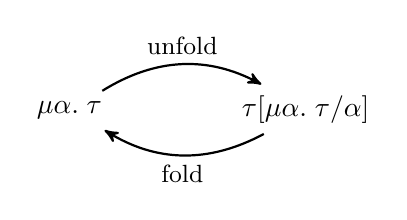
\begin{tikzpicture}[->,>=stealth',shorten >=1pt,auto,node distance=3cm,
  thick,main node/.style={rectangle}]

  \node[main node] (1) {$\mu\alpha.\; \tau$};
  \node[main node] (2) [right of=1] {$\tau[\mu \alpha. \; \tau / \alpha]$};

  \path[every node/.style={font=\sffamily\small}]
    (1) edge [bend left] node [above] {$\unfold$} (2)
    (2) edge [bend left] node [below] {$\fold$} (1);
\end{tikzpicture}
\]
With recursive types in hand we can now define our tree type:
\[
  tree \eqdef \mu \alpha. \; 1 + (int \times \alpha \times \alpha)
\]
When we want to work with this, we would like to be able to get under the $\mu$. Say we have $e : tree$ that is an expression $e$ with type $tree$, then we want to be able to say whether it is a leaf or a node. To do so we unfold the type to get the type where $\alpha$ has been substituted with the definition of $tree$ and the outer $\mu\alpha.$ has been removed. With the outer $\mu\alpha.$ gone we can match on the sum type to find out whether it is a leaf or a node. We can fold the type back to the original tree type, when we are done working with it.
\[
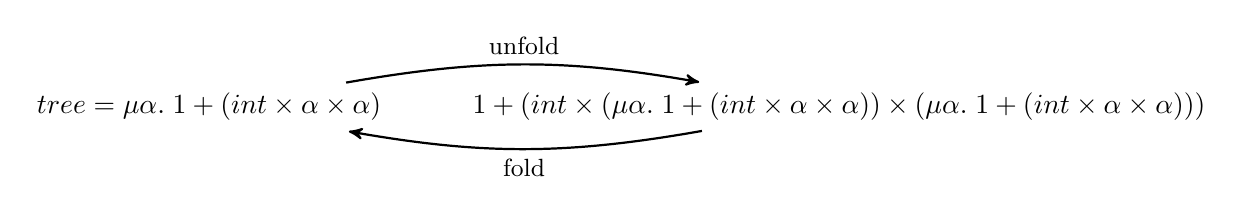
\begin{tikzpicture}[->,>=stealth',shorten >=1pt,auto,node distance=3cm,
  thick,main node/.style={rectangle}]

  \node[main node] (1) {$tree=\mu\alpha.\; 1+(int \times \alpha \times \alpha)$};
  \node[main node] (2) [right of=1,xshift=5cm] {$1+(int \times (\mu\alpha.\; 1+(int \times \alpha \times \alpha)) \times (\mu\alpha.\; 1+(int \times \alpha \times \alpha)))$};

  \path[every node/.style={font=\sffamily\small}]
    (1) edge [bend left=10] node [above] {$\unfold$} (2)
    (2) edge [bend left=10] node [below] {$\fold$} (1);
\end{tikzpicture}
\]
This kind of recursive types is called iso-recursive types, because there is an isomorphism between a $\mu\alpha. \; \tau$ and its unfolding $\tau[\mu\alpha.\; \tau / \alpha]$. 

STLC extended with recursive types is defined as follows:
\begin{align*}
  \tau &::= \dots \vbar \mu \alpha. \; \tau \\
  e    &::= \dots \vbar \fold \; e \vbar \unfold \; e \\
  v    &::= \dots \vbar \fold \; v\\
  E    &::= \dots \vbar \fold \; E \vbar \; \unfold \; E
\end{align*}
\[
\unfold \; (\fold \; v) \evalto v
\]
\[
\TFold \hspace{2cm} \TUnfold
\]
With this we could define the type of an integer list as:
\[
int\; list \eqdef \mu\alpha.\; 1 + (int \times \alpha)
\]
%TODO: Typing omega
\begin{comment}
\[
  \Omega = (\tlabs{x}{\mu\alpha.\; \tarrow{\alpha}{\tau}}{(\unfold \; x) \; x}) 
\]
\end{comment}
\subsection*{Exercises}
\begin{enumerate}
\item Prove the TApp case of the Fundamental Property
\end{enumerate}
\clearpage


\section*{Lecture 3, Step-Indexing}
This lecture was on extending the unary logical relation for type safety of simply typed lambda calculus to recursive types, introducing universal types, and finally a short introduction to contextual equivalence.

\subsection*{Simply typed lambda calculus extended with $\mu$}
In a naive first attempt to make the value interpretation we could write something like
\[
  \vpred{\mu\alpha. \; \tau} = \{\fold \; v \vbar \unfold \; (\fold \; v) \in \epred{\sub{\tau}{\mu\alpha.\;\tau}{\alpha}} \}
\]
We can simplify this slightly; first we use the fact that $\unfold \; (\fold \; v)$ reduces to $v$. Next, we use the fact that $v$ must be a value and the fact that we want $v$ to be in the expression interpretation of $\tau[\mu \alpha. \; \tau / \alpha]$. By unfolding the definition of the expression interpretation we conclude that it suffices to require $v$ to be in the value interpretation of the same type. We then end up with the following definition:
\[
  \vpred{\mu\alpha. \; \tau} = \{\fold \; v \vbar v \in \vpred{\sub{\tau}{\mu\alpha.\;\tau}{\alpha}} \}
\]
This gives us a well-foundness issue. The value interpretation is defined by induction on the type, $\sub{\tau}{\mu\alpha.\;\tau}{\alpha}$ is not a structurally smaller type than $\mu\alpha. \; \tau$. 

To solve this issue we index the interpretation by a natural number which we write as follows:
\[
  \vpres{\tau} = \{v \vbar \dots \}
\]
If $v$ belongs to the interpretation, then this is read as ``$v$ belongs to the interpretation of $\tau$ for $k$ steps.'' We interpret this in the following way; given a value that we run run for $k$ or fewer steps as in the value is used in some program context for $k$ or fewer steps, then we will never notice that it does not have type $\tau$. If we use the same value in a program context that wants to run for more than $k$ steps, then we might notice that it does not have type $\tau$ which means that we might get stuck. This gives us an approximate guarantee.

We use this as an inductive metric to make our definition well-founded, so we define the interpretation on induction on the step-index followed by inner induction on the type structure. Let us start by adding the step-index to our existing value interpretation:
\begin{align*}
  \vpres{bool} &= \{\true,\false\} \\
  \vpres{\tarrow{\tau_1}{\tau_2}} &= \{\tlabs{x}{\tau_1}{e} \vbar \forall j \leq k. \; \forall v \in \vpres[j]{\tau_1}. \; \sub{e}{v}{x} \in \epres[j]{\tau_2} \}
\end{align*}
$\true$ and $\false$ are in the value interpretation of $bool$ for any $k$, so $\true$ and $\false$ will for any $k$ look like it has type $bool$. To illustrate how to understand the value interpretation of $\tarrow{\tau_1}{\tau_2}$ please consider the following timeline:  \\
\begin{center}
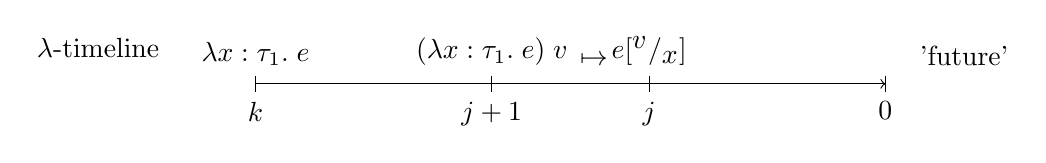
\begin{tikzpicture}
    % draw horizontal line   
    \draw[->] (0,0) -- (8,0);

    % draw vertical lines
    \foreach \x in {0,3,5,8}
      \draw (\x cm,3pt) -- (\x cm,-3pt);

    % draw nodes
    \draw (-2,0) node[below=3pt] {  } node[above=6pt] {$\lambda$-timeline};
    \draw (0,0) node[below=3pt] {$k$} node[above=3pt] {$ \tlabs{x}{\tau_1}{e}$};
    \draw (3,0) node[below=3pt] {$ j+1 $} node[above=3pt] {$(\tlabs{x}{\tau_1}{e})\; v $};
    \draw (4.3,0) node[below=3pt] {$   $} node[above=3pt] {$ \evalto $};    
    \draw (5,0) node[below=3pt] {$ j $} node[above=3pt] {$ \sub{e}{v}{x} $};
    \draw (8,0) node[below=3pt] {$ 0 $} node[above=3pt] {$  $};
    \draw (9,0) node[below=3pt] {$   $} node[above=3pt] { 'future' };
  \end{tikzpicture}
\end{center}
Here we start at index $k$ and as we run the program we use up steps until we at some point reach 0 and rund out of steps. At step $k$ we are looking at a lambda. A lambda is used by applying it, but it is not certain that the application will happen right away, as the we only do $\beta$-reduction when we try to apply a lambda to a value, but we might be looking at a context where we want to apply the lambda to an expressions, i.e.\ $(\tlabs{x}{\tau_1}{e})\; e_2$. We might use a bunch of steps to reduce $e_2$ down to a value, but we cannot say how many. So say that sometime in the futurewe have fully evaluated $e_2$ to $v$ and say that we have $j+1$ steps left at this time, then we can do the $\beta$ reduction which gives us $\sub{e}{v}{x}$ at step $j$. % If we ever hit 0 steps, then all bets are off. the value can have any type.

We can now define the value interpretation of $\mu\alpha. \; \tau$:
\[
  \vpres{\mu\alpha.\; \tau} = \{\fold \; v \vbar \forall j < k. \; v \in \vpres[j]{\tau\sub{\mu\alpha.\;\tau}{\alpha}} \}
\]
This definition is like the one we previously proposed, but with a step-index. This definition is well-founded because $j$ is required to be \emph{strictly} less than $k$ and as we define the interpretation on induction over the step-index this is indeed well founded. We do not define a value interpretation for type variables $\alpha$, as we have no polymorphism yet. The only place we have a type variable at the moment is in $\mu\alpha. \; \tau$, but in the interpretation we close of the $\tau$ under the $\mu$, so we will never encounter a free type variable.

Finally, we define the expression interpretation:
\[
  \epres{\tau} = \{e \vbar \forall j < k. \; \forall e'. \; e \evaltos[j] e' \; \wedge \; \irred(e') \; \implies \; e' \in \vpres[k-j]{\tau}\}
\]
To illustrate what is going on here consider the following timeline: \\
\begin{center}
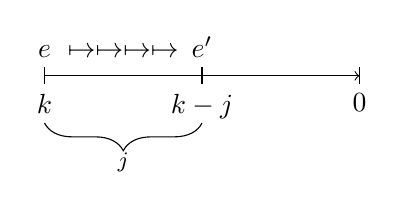
\begin{tikzpicture}
    % draw horizontal line   
    \draw[->] (0,0) -- (4,0);

    % draw vertical lines
    \foreach \x in {0,2,4}
      \draw (\x cm,3pt) -- (\x cm,-3pt);

    % draw nodes
    \draw (0,0) node[below=3pt] {$k$} node[above=3pt] {$e$};
    \draw (1,0) node[below=3pt] {$ $} node[above=3pt] {$\evalto \evalto \evalto \evalto$};
    \draw (2,0) node[below=3pt] {$k-j$} node[above=3pt] {$e'$};
    \draw (4,0) node[below=3pt] {$0$} node[above=3pt] {$  $};

    % brace
    \draw [decorate,decoration={brace,amplitude=10pt,mirror}]
    (0,-0.6) -- (2,-0.6) node [black,midway,yshift=-0.5cm] 
          {\footnotesize $j$};
\end{tikzpicture}
\end{center}
We start with an expression $e$, then we take $j$ steps and get to expression $e'$. At this point if $e'$ is irreducable, then we want it to belong to the value interpretation of $\tau$ for $j-k$ steps. The reason we use a strict inequality is that we do not want to hit 0 steps. If we hit 0 steps, then all bets are off.%TODO: why are all bets off?

We also need to lift the interpretation of type environments to step-indexing:
\begin{align*}
  \gpres{\mtenv} & = \{\emptyset \} \\
  \gpres{\Gamma, x : \tau} & = \{ \gamma[x \mapsto v] \vbar \gamma \in \gpres{\Gamma} \; \wedge \; v \in \vpres{\tau} \}
\end{align*}

\[
  \Gamma \models e : \tau \eqdef \forall k \geq 0. \; \forall \gamma \in \gpres{\Gamma} \; \implies \gamma(e) \in \epres{\tau}
\]

\begin{stlcmufundprop}[Fundemental property]
  If $\Gamma \vdash e : \tau$ then $\Gamma \models e : \tau$.
\end{stlcmufundprop}

\[
\circled{b} \quad \mtenv \models e : \tau \implies \safe(e)
\]

\begin{monotonicity}
  If $v\in \vpres{\tau}$ and $j \leq k$  then $v \in \vpres[j]{\tau}$.
\end{monotonicity}
\begin{proof}
We prove this by case on $\tau$.
\case{$\tau = bool$}
assume $v \in \vpres{bool}$ and $j \leq k$, we then need to show $v \in \vpres[j]{bool}$. As $v \in \vpres{bool}$ we know that either $v= \true$ or $v=\false$. If we assume $v=\true$, then we immidiately get what we want to show, as $\true$ is in $\vpres[j]{bool}$ for any $j$. Likewise for the case $v=\false$.
\case{$\tau = \tarrow{\tau_1}{\tau_2}$}
assume $v \in \vpres{\tarrow{\tau_1}{\tau_2}}$ and $j \leq k$, we then need to show $v \in \vpres[j]{\tarrow{\tau_1}{\tau_2}}$. As $v$ is a member of $\vpres{\tarrow{\tau_1}{\tau_2}}$ we can conclude that $v = \tlabs{x}{\tau_1}{e}$ for some $e$. By definition of $v \in \vpres[j]{\tarrow{\tau_1}{\tau_2}}$ we need to show $\forall i \leq j. \forall v' \in \vpres[i]{\tau_1}.\; v' \in \epres[i]{\tau_2}$. Suppose $i \leq j$ and $v' \in \vpres[i]{\tau_1}$, we then need to show $v' \in \epres[i]{\tau_2}$.

By assumption we have $v \in \vpres{\tarrow{\tau_1}{\tau_2}}$ which gives us $\forall n \leq k. \forall v' \in \vpres[n]{\tau_1}.\; v' \in \epres[n]{\tau_2}$. From $j \leq k$ and $i \leq j$ we get $i \leq k$ by transitivity. We use this with $v' \in \vpres[i]{\tau_1}$ to get $v' \in \epres[i]{\tau_2}$ which is what we needed to show.
\case{$\tau = \mu \alpha.\; x$}
assume $v \in \vpres{\mu\alpha. \; \tau}$ and $j \leq k$, we then need to show $v \in \vpres[j]{\mu\alpha. \; \tau}$. From $v$'s assumed membership of the value interpretation of $\tau$ for $k$ steps we conclude that there must exist a $v'$ sucht that $v = \fold \; v'$. If we suppose $i<j$, then we need to show $v' \in \vpres[i]{\subst{\tau}{\mu\alpha.\; \tau}{\alpha}}$. From $i<j$ and $j \leq k$ we can conclude $i < k$ which we use with $\forall n < k.\; v' \in \vpres[n]{\subst{\tau}{\mu\alpha.\; \tau}{\alpha}}$, which we get from $v \in \vpres{\mu\alpha. \; \tau}$, to get $v' \in \vpres[i]{\subst{\tau}{\mu\alpha.\; \tau}{\alpha}}$.
\end{proof}

\begin{proof}[Proof (Fundemental Property)]
  
\end{proof}

\[
  \vpres{\tau_1 + \tau_2} = \{\inl \; v_1 \vbar v_1 \in \vpres{\tau_1}\} \cup 
                            \{\inr \; v_2 \vbar v_2 \in \vpres{\tau_2}\}
\]

\subsection*{Universal Types}
\[
  sort \; : \; \forall \alpha.\; \tarrow{(list \; \alpha) \times (\tarrow{\alpha \time \alpha}{bool} )}{list \; \alpha}
\]
\[
  sort[int](3,5,7)<
\]
\[
  \tLabs{e}
\]

\subsubsection*{System F (Simply Typed Lambda Calculus With Universal Types)}
\begin{align*}
  \tau &::= \dots \vbar \forall \alpha. \; \tau \\
  e    &::= \dots \vbar \tLabs{e} \vbar e[\tau] \\
  v    &::= \dots \vbar \tLabs{e}\\
  E    &::= \dots \vbar \fold \; E[\tau] 
\end{align*}
\[
  (\tLabs{e}[\tau]) \evalto e[\tau/\alpha]
\]
Type environment
\[
  \Delta ::= \mtenv \vbar \Delta,\; \alpha
\]
Type judegement form:
\[
  \Delta,\Gamma \vdash e : \tau
\]
Well formed type:
\[
  \Delta \vdash \tau \eqdef \FTV(\tau) \subseteq \Delta
\]
where $\FTV(\tau)$ is the set of free type variables in $\tau$.

Well-formed environment
\[
  \Delta \vdash \Gamma \eqdef \forall x \in \dom(\Gamma). \; \Delta \vdash \Gamma(x)
\]
For any type judgement $\Delta,\Gamma \vdash e : \tau$ we have as an invariant that $\Delta \vdash \Gamma$.
Typing rules:
\[
  \FTFalse
\hspace{1cm}
  \FTTrue
\]
\[
  \FTVar
\hspace{1cm}
  \FTIf
\]  
\[
  \FTAbs 
\hspace{1cm}
  \FTApp
\]

\begin{theorem}
  If $\mtenv ; \mtenv \vdash e : \forall \alpha. \; \tarrow{\alpha}{\alpha}$,\\ $\mtenv \vdash \tau$, and\\ $\mtenv; \mtenv \vdash v : \tau$\\ then $e[\tau]\; v \evaltos v$
\end{theorem}

\subsection*{Exercises}
\begin{enumerate}
\item Do the lambda and application case of the \emph{Fundemental Property} theorem.%Specify in what proof, probably fundemental property
\item Try to prove the monotonicity lemma where the definition of the value interpretation has been adjusted with:
\[
\vpres{\tarrow{\tau_1}{\tau_2}} = \{\tlabs{x}{\tau_1}{e} \vbar \; \forall v \in \vpres{\tau_1}. \; \sub{e}{v}{x} \in \epres{\tau_2} \}
\]
This will fail, but it is instructive to see how it fails.
\end{enumerate}


%induction on step index followed by inner induction on the type structure.
%when an expression looks like it has type tau.
\clearpage

\section*{Lecture 4}

\clearpage

\section*{Lecture 5}

\clearpage

\section*{Acknowledgments}
It is established practice for authors to accept responsibility for
any and all mistakes in documents like this. I, however, do not. If
you find anything amiss, please let me know so I can figure out who of
the following are to blame: Amal Ahmed, Morten Krogh-Jespersen or
Kristoffer Just Andersen.
\end{document}
